\graphicspath{{./figures}}

\section{Antennas}

There are various antenna types to consider for this communication system. A highly-customized antenna design is out of the scope of this project, and therefore only common, existing designs with tunable parameters will be considered. These antennas should also be compared in the context of the UHF frequencies of interest (400 MHz to 440 MHz). Ultimately, the following characteristics will be used to compare the various options:
\begin{itemize}
    \item Radiation pattern (qualitative shape)
    \item Gain (relative to an \textit{isotropic} source) 
    \item Bandwidth (relative to resonant frequency)
    \item Beamwidth (width of \textit{main lobe})
    \item Dimensions
\end{itemize}

\subsection{Half-Wave Dipole}
\begin{figure}[!htb]
  \centering
  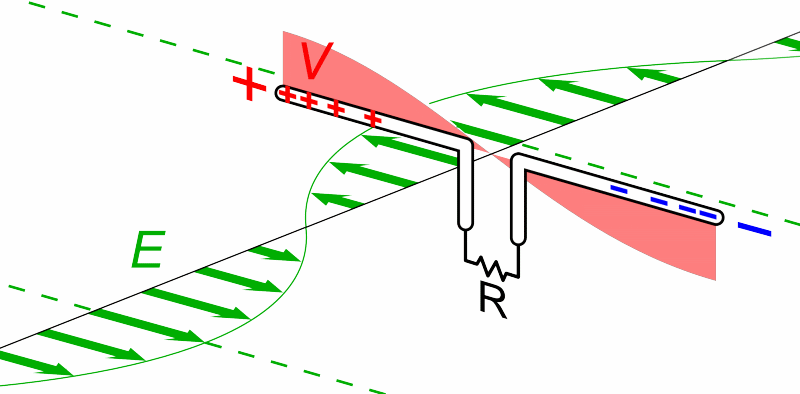
\includegraphics[width=0.4\textwidth]{dipole}
  \caption{Dipole Antenna Illustration \cite{site-designingDipole}}
  \label{fig:dipole}
\end{figure}

The half-wavelength ($0.5 \lambda$) dipole anntenna is arguably the simplest and most common type of antenna. It consists of two conductive elements operating in opposite phase, as depicted in Figure \ref{fig:dipole}. It is considered \textit{omni-directional} i.e. it radiates relatively equally in all directions. Its gain is relatively low, at around 2.15 dBi \cite{site-antennaTheory}. Further, it does not radiate in the direction of the conductor.

\subsection{General Dipole}
Dipole antennas can, in general, be any length. However, a change in length results in a change in the antenna's characteristics. In general, smaller antennas result in lower gain and lower efficiency, but a larger beamwidth at the resonant frequency. The obvious advantage of these designs is that the size of the dipole can be decreased. However, if size is a constraint, \textit{monopole} antennas are generally employed.

\subsection{Quarter-Wave Monopole}
The working principle of monopole antennas makes use of the electromagnetic theory of \textit{imaging}. Essentially, if an infinite ground plane is placed below one half of a $0.5 \lambda$ dipole antenna, then the electromagnetic waves react with the ground plane in a way which causes propogation similar to a half-wavelength dipole. They are extremely useful when size is a constraint, however have the disadvantage of requiring a ground plane. A \textit{whip} antenna is a form of monopole antenna designed to be flexible so that it does not break as easily, and often placed inside a plastic enclosure, as in Figure \ref{fig:whip}.

\begin{figure}[!htb]
  \centering
  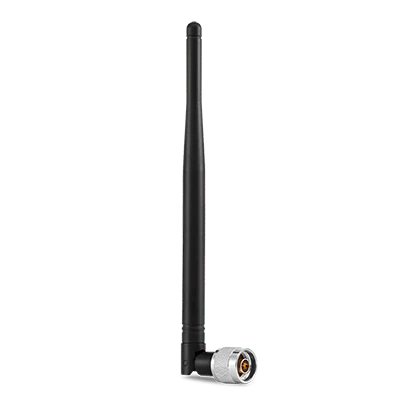
\includegraphics[width=0.3\textwidth]{whip}
  \caption{Whip Antenna in Plastic Housing}
  \label{fig:whip}
\end{figure}

\subsection{Helical}
\begin{figure}[!htb]
  \centering
  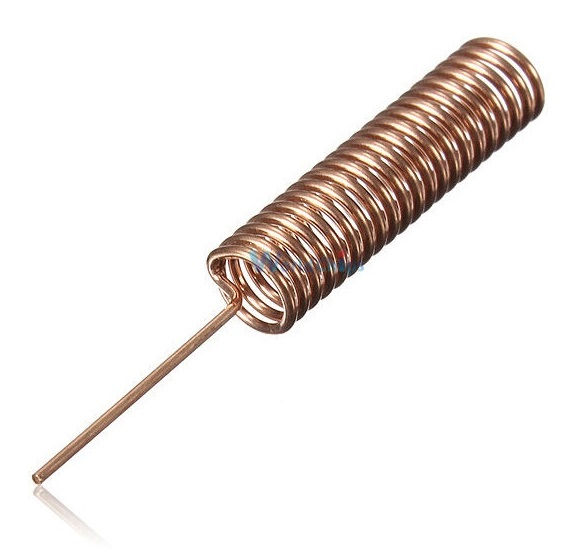
\includegraphics[width=0.2\textwidth]{helical_uni}
  \caption{Helical, Unidirectional Antenna}
  \label{fig:helical_uni}
\end{figure}

Helical antennas are coiled windings of wire, where the circumference of the coil has some direct relationship with the desired wavelength. Commonly, a circumference of $C = 1.0 \lambda$ is used. Both \textit{omni-directional} and \textit{unidirectional} variants are possible, with the latter having an extended \textit{feedline}, as shown in Figure \ref{fig:helical_uni}. These antennas have the major advantage of a small size, due to the \textit{circumference} being related to the wavelength as opposed to the antennas length itself. Further, they have several design parameters that can influence the antennas functionality, such as number of turns, wire width, and turn pitch angle. They also are able to receive either linear or circularly polarized signals, making them more flexible.


\subsection{Patch}
A \textit{patch} antenna (also known as a \textit{PCB} antenna) is simply a rectangular PCB trace sized correctly to allow for radiation. Typically, a simple square or rectangular shape can be used. They allow for extremely small profiles at the cost of efficiency \cite{site-antennaTheory}, and can be integrated onto a PCB using normal trace techniques.

\subsection{Array}
It should be noted that multiple antennas can be combined in what is known as an \textit{array} configuration. This allows complete manipulation of the design due to \textit{constructive} and \textit{destructive} interference, meaning directivity can be increased or decreased. Common variations of this concept reside in \textit{Yagi-Uda} and \textit{Patch Array} antennas.

\subsection{Yagi-Uda}
\begin{figure}[!htb]
  \centering
  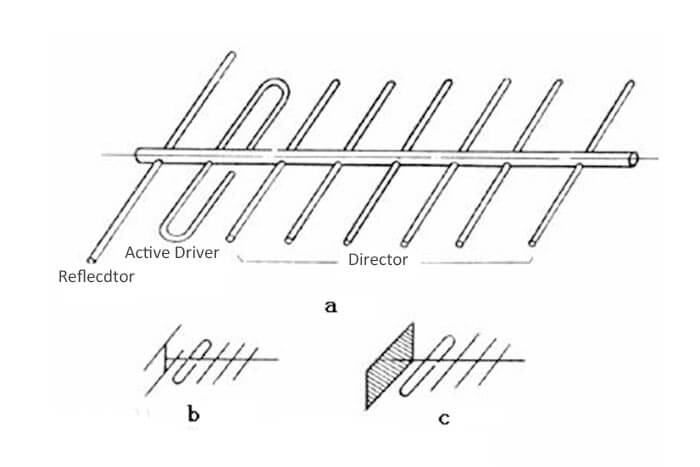
\includegraphics[width=0.4\textwidth]{yagi}
  \caption{Yagi-Uda Antenna \cite{site-icantennasYagi}}
  \label{fig:yagi}
\end{figure}
Although not strictly an antenna array, \textit{Yagi-Uda} antennas are one of the most popular directive antennas available. A number of conductors are stacked in a specific configuration to "steer" the electromagnetic waves using interference. Only one of the conductors in the array is actually fed with a signal - the rest are merely \textit{passive} elements used for increasing the directivity. An example of such an antenna is shown in Figure \ref{fig:yagi}.

\subsection{Modified Patch}
\begin{figure}[!htb]
  \centering
  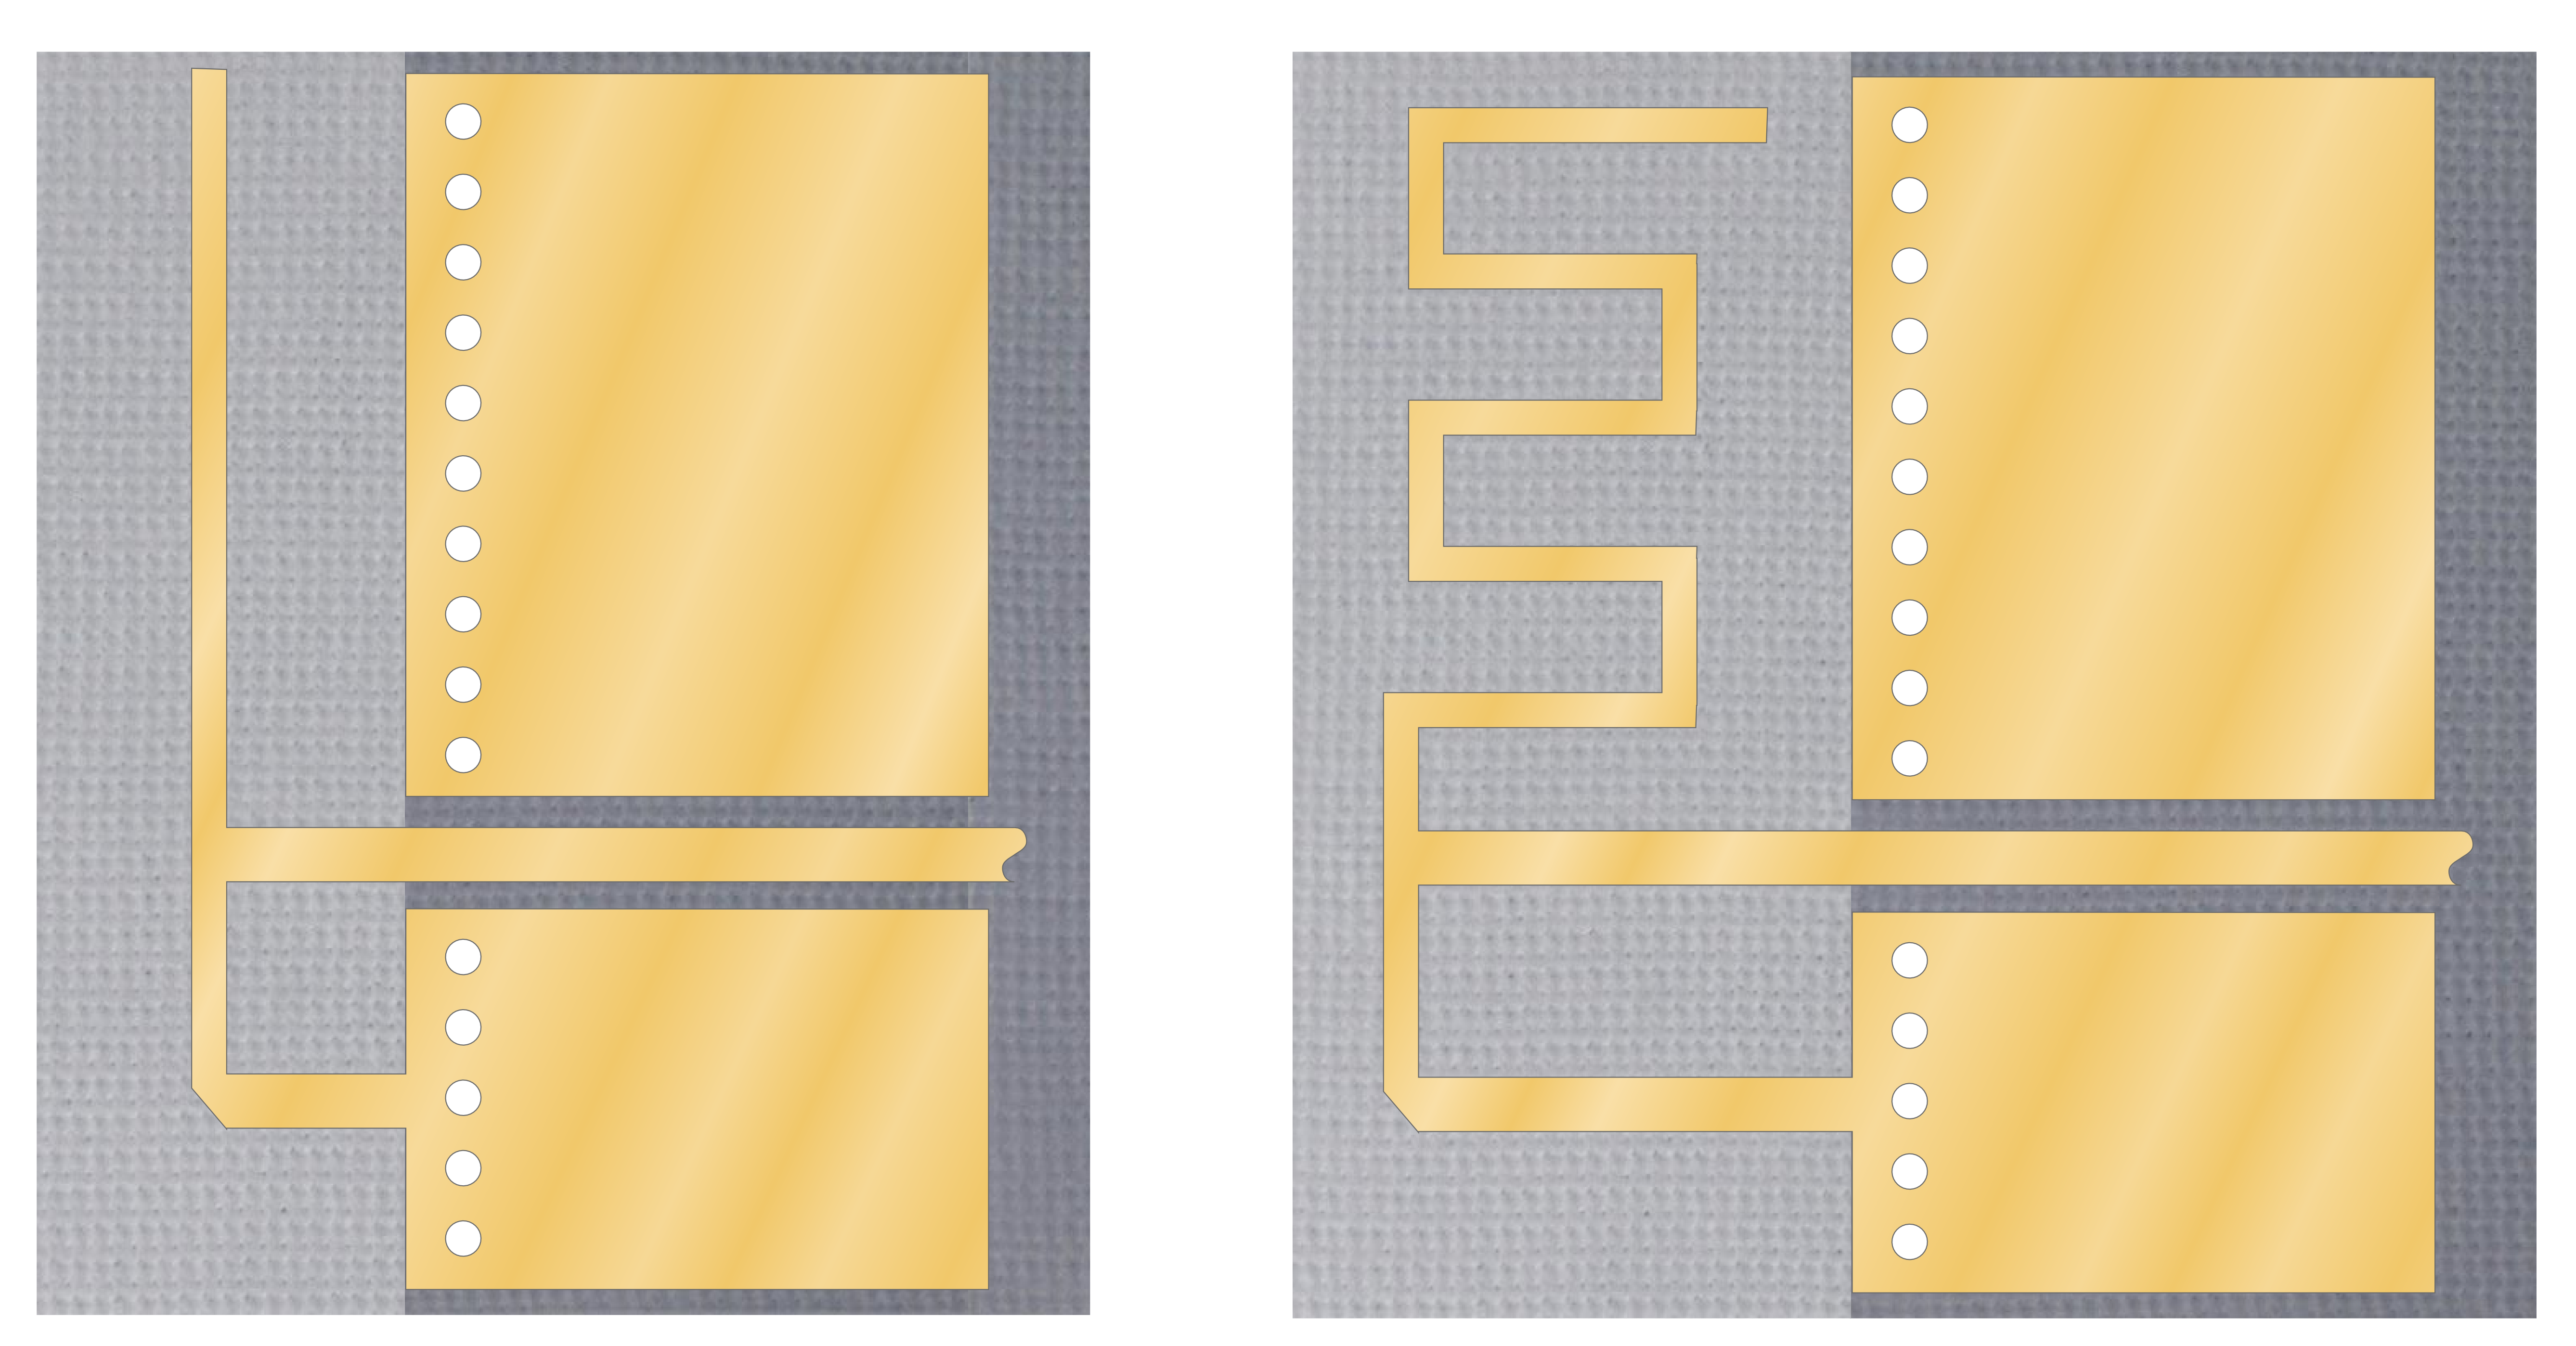
\includegraphics[width=0.3\textwidth]{invertedF}
  \caption{Inverted-F Patch Antennas \cite{site-invertedFAntenna}}
  \label{fig:invertedF}
\end{figure}
Several modified designs exist for patch antennas which allow for varying characteristics. Although many of these designs originated from non-PCB antenna designs, their complexity is mostly on justified when implemented on a flat PCB for a non-antenna focused projected. Examples include a \textit{patch array}, which allows for a increased directivity, or an \textit{inverted-F} design, which allows for much smaller form factorer and a nearly full 3D omni-directional radiation pattern. A multi-frequency version of the latter is illustrated in Figure \ref{fig:invertedF}. A third example is a \textit{helical patch} antenna, which is simply a "zig-zag" helical shape flattened onto a PCB.

\subsection{Summary}

The following table presents a general summary of the investigated antennas. Note that a number of these parameters can vary due to the design (e.g. a thicker dipole results in larger bandwidth), however typical values have been chosen for an initial comparison. A thickness of 1mm has been chosen arbitrarily for dimensions which do not contribute to an antenna's form factor. 

\begin{table}[!htb]
  \centering
  \hspace*{-2cm}
  \renewcommand{\arraystretch}{1.2}
  \begin{tabular}{ |c|c|c|c|c|c| }
  \hline
  \textbf{Type} & \textbf{Gain (dBi)} & \textbf{Radiation} & \textbf{Bandwidth (frac.)} & \textbf{Beamwidth (\textdegree)} & \textbf{Dimensions (mm)} \\ \hline
  $0.5 \lambda$ Dipole & 2.15 & Omnidirectional & 0.1 & 78 & 1 x 1 x 172 \\ \hline
  Whip & 1.76 & Omnidirectional & 0.1 & 78 & 1 x 1 x 86 \\ \hline
  Helical & 2-10 & Either & 0.56 & 60 & 4.4 x 4.4 x 25 \\ \hline
  Patch & 5-7 & Unidirectional & 0.03 & 65 & 346 x 346 x 1 \\ \hline
  Yagi-Uda & 10+ & Unidirectional & 0.02 & 30-60 & 172 x 1 x 500+ \\ \hline
  \end{tabular}
  \caption{Comparison of Common Antennas and their Typical Characteristics \cite{site-antennaTheory}}
  \label{tab:antenna_characteristics}
\end{table}